\section{Evaluation}

% TODO: Compare against some P4 programs, for instance, flowlet switching and HULA.

\label{s:eval}

\begin{table}[!t]
  \begin{scriptsize}
  \begin{tabular}{|p{0.1\textwidth}|p{0.23\textwidth}|p{0.1\textwidth}|}
    \hline
    Atom & Description & Area in square microns \\
    \hline
    Read/Write & Read/Write packet field/constant into single state variable. & 249 \\
    \hline
    ReadAddWrite (RAW) & Add packet field/constant to state variable (OR) Write packet field/constant into state variable. & 430 \\
    \hline
    Predicated ReadAddWrite (RAW) & Execute RAW on state variable only if a predicate is true, else leave unchanged. & 790 \\
    \hline
    IfElse ReadAddWrite (IfElseRAW) & Execute two separate RAWs: one each for when a predicate is true or false. & 985 \\
    \hline
    Subtract (Sub) & Same as IfElseRAW, but also allow subtracting a packet field/constant. & 1301 \\
    \hline
    Nested Ifs (Nested) & Same as Sub, but with an additional level of nesting that provides 4-way predication. & 3091 \\
    \hline
    Paired updates (Pairs) & Same as Nested, but allow updates to a pair of state variables, where predicates can use both state variables. & 4440 \\
    \hline
  \end{tabular}
  \end{scriptsize}
  \caption{Stateful atoms, along with their area overhead in a 32 nm standard-cell library.
    All atoms meet timing at 1GHz. Appendix A provides the SKETCH code and
  circuit diagrams for these atoms.}
  \label{tab:templates}
\end{table}

\begin{table}[!t]
  \begin{scriptsize}
    \begin{tabular}{|p{0.08\textwidth}|p{0.29\textwidth}|p{0.04\textwidth}|}
  \hline
  Atom & Circuit & Element depth \\
  \hline
  Write & 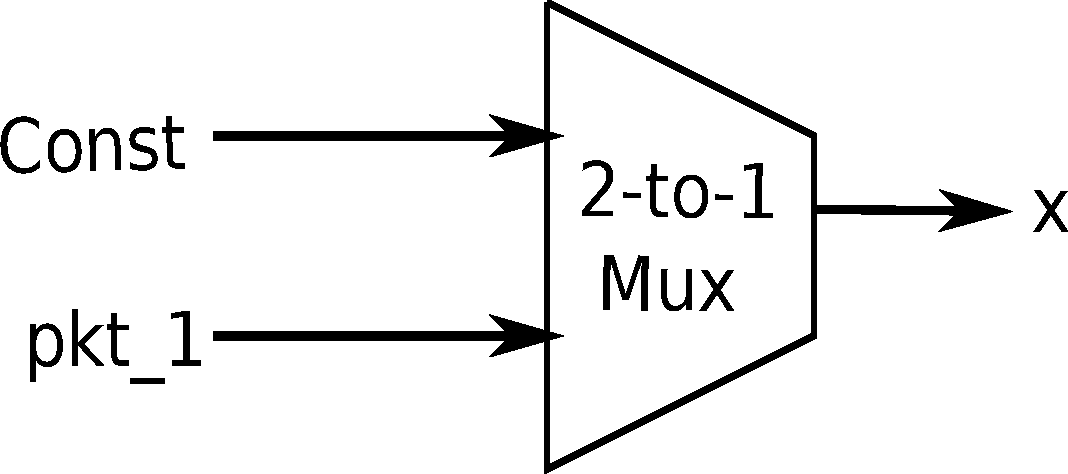
\includegraphics[width=0.2\textwidth]{rw.pdf} & 1 \\
  \hline
  ReadAddWrite (RAW) & 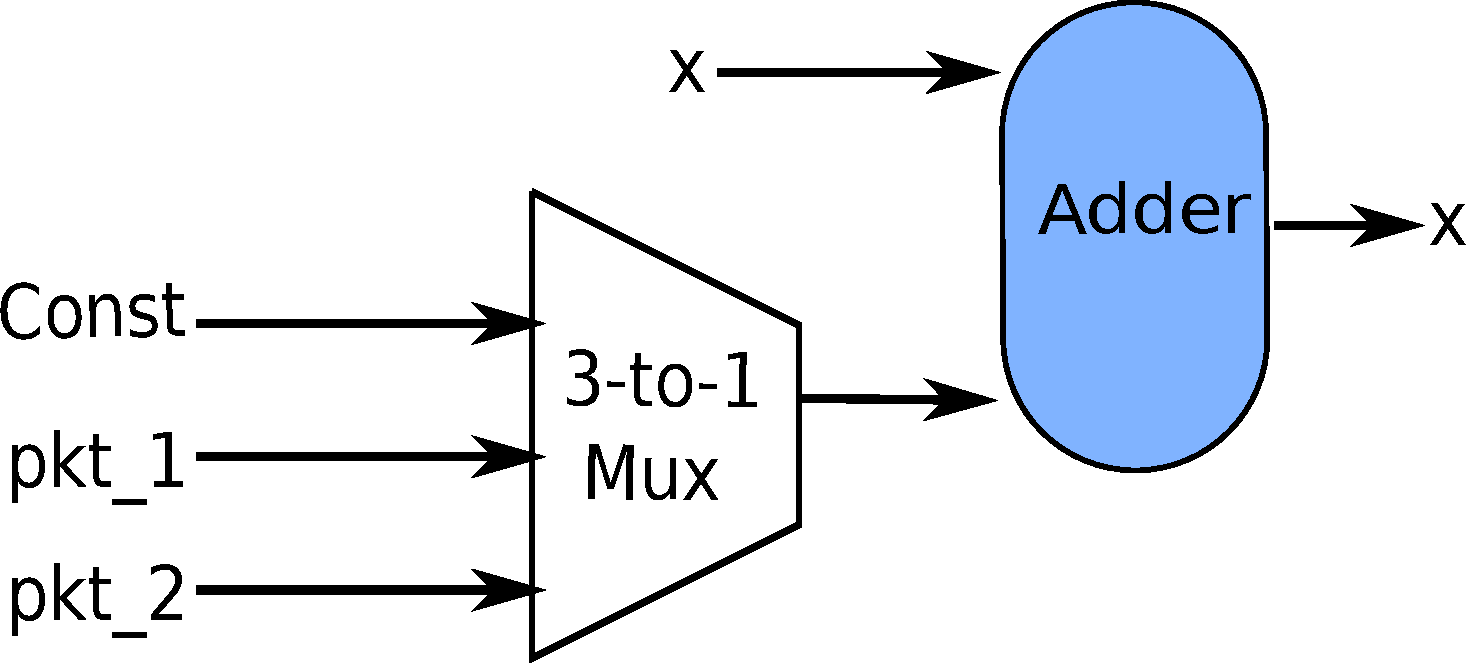
\includegraphics[width=0.2\textwidth]{raw.pdf} & 2\\
  \hline
  \pbox{0.1\textwidth}
  {Predicated\\
  ReadAddWrite (PRAW)} & 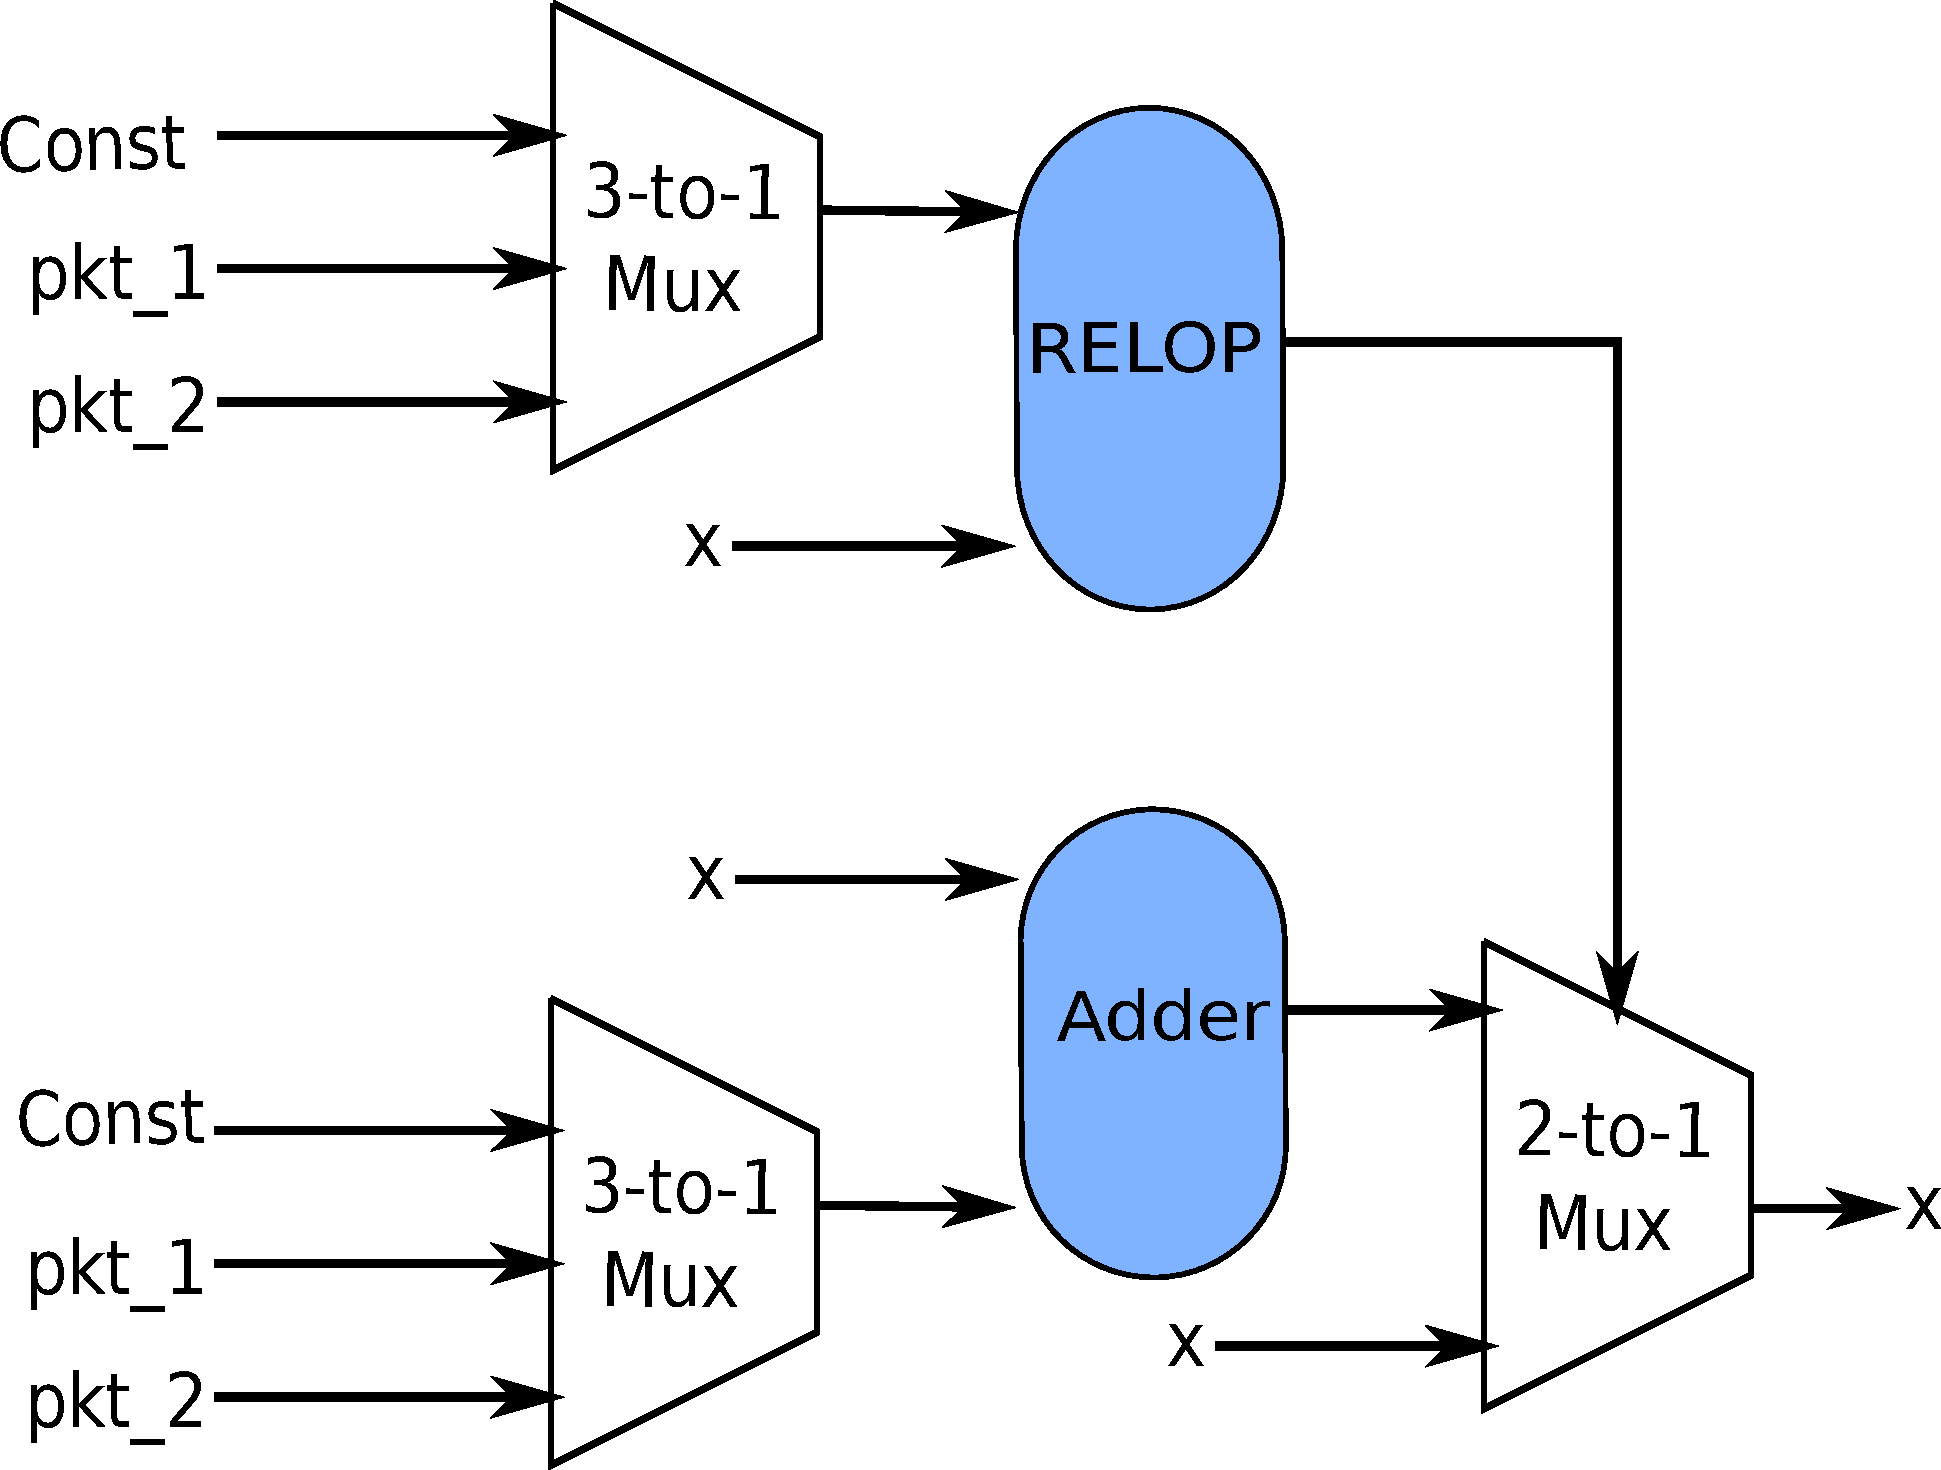
\includegraphics[width=0.3\textwidth]{pred_raw.pdf}  & 3\\
  \hline
  \end{tabular}
\end{scriptsize}
\caption{Element depth and propagation delay increases with complexity of atoms.}
  \label{fig:element_depth}
\end{table}

\begin{table*}[!t]
  \begin{tabular}{|p{0.16\textwidth}|p{0.47\textwidth}|p{0.09\textwidth}|p{0.06\textwidth}|p{0.07\textwidth}|}
\hline
Algorithm & Stateful computation & Least expressive atom & Pipeline depth, width & Ingress or Egress Pipeline?\\
\hline
\pbox{0.16\textwidth}{Bloom filter~\cite{bloom}\\(3 hash functions)} & \pbox{0.54\textwidth}{Set membership bit on every packet.} & Write & 4, 3 & Either \\
\hline
\pbox{0.16\textwidth}{Heavy Hitters~\cite{opensketch}\\(3 hash functions)} & Increment Count-Min Sketch~\cite{cormode} on every packet. & RAW & 10, 9 & Either \\
\hline
Flowlets~\cite{flowlets} & Update saved next hop if flowlet threshold is exceeded. & PRAW & 6, 2 & Ingress \\
\hline
RCP~\cite{rcp} & \pbox{0.47\textwidth}{Accumulate RTT sum if\\RTT is under maximum allowable RTT.} & PRAW & 3, 3 & Egress \\
\hline
\pbox{0.16\textwidth}{Sampled\\NetFlow~\cite{sampled_nflow}} & \pbox{0.47\textwidth}{Sample a packet if packet count reaches N;\\Reset count to 0 when it reaches N.} & IfElseRAW & 4, 2 & Either\\
\hline
HULL~\cite{hull} & Update counter for virtual queue. & Sub & 7, 1 & Egress \\
\hline
\pbox{0.16\textwidth}{Adaptive\\Virtual Queue~\cite{avq}} & Update virtual queue size and virtual capacity & Nested & 7, 3 & Ingress \\
\hline
CONGA~\cite{conga} & \pbox{0.54\textwidth}{Update best path's utilization/id if we see a better path.\\
                                           Update best path utilization alone if it changes.}  & Pairs & 4, 2 & Ingress\\
\hline
trTCM~\cite{trTCM} & Update token counts for each token bucket & Doesn't map & 7, 3 & Either \\
\hline
CoDel~\cite{codel} & \pbox{0.54\textwidth}{Update:\\Whether we are marking or not.\\Time for next mark.\\Number of marks so far.\\Time at which min. queuing delay will exceed target.}& Doesn't map & 15, 3 & Egress \\
\hline
\end{tabular}
\caption{Data-plane algorithms}
\label{tab:algos}
\end{table*}

We evaluate \pktlanguage's expressiveness by using it to express several
data-plane algorithms (Table~\ref{tab:algos}). We then design a set of
\absmachine machines (Table~\ref{tab:templates}) that serve as compiler targets
for \pktlanguage.  These machines are readily feasible in today's transistor
technology and their atoms incur modest area overhead relative to a baseline
switching chip. Next, we use the \pktlanguage compiler to compile the programs
in Table~\ref{tab:algos} to the targets in Table~\ref{tab:templates}.  We
conclude by quantitatively demonstrating a tradeoff between a target's
programmability (the space of data-plane algorithms that it can run at line
rate) and the target's performance (the maximum line rate it can support).

\subsection{Expressiveness}
\label{ss:Expressiveness}

To evaluate \pktlanguage's expressiveness, we express several data-plane
algorithms (Table~\ref{tab:algos}) in \pktlanguage. These algorithms encompass
a variety of data-plane functionality: data-plane load balancing, in-network
congestion control, active queue management, and measurement. In addition,
\pktlanguage has been used for programmable scheduling~\cite{prog_sched_arxiv}.
In all these cases, the algorithms are naturally expressed as blocks of
imperative code. Expressing an algorithm in \pktlanguage involved a
straightforward translation of the algorithm's reference code/pseudo code to
\pktlanguage.
%TODO: Maybe add a few examples from Chimera/Bohatei on security.

By contrast, expressing one of these algorithms in a language like P4---as one
would today---requires manually teasing out portions of the algorithm that can
reside in independent match-action tables and then chaining these tables
together to implement the algorithm---in essence, manually carrying out the
transformations in \pktlanguage's compiler.

\paragraph{Quantitative comparison against P4}
Of the algorithms in Table~\ref{tab:algos}, only flowlet switching has a
hand-written P4 implementation today~\cite{p4_flowlet}. This implementation
requires 292 lines of uncommented P4, in comparison to the 32 lines of
\pktlanguage in Figure~\ref{fig:flowlet_code}. Further, the same implementation
only runs on a software switch because it requires synchronized access to the
saved\_hop variable from two adjacent pipeline stages---something that is very
challenging on shared-nothing line-rate switches. This illustrates the
additional cognitive overhead when programming with P4: reasoning about how
state variables are distributed across a pipeline is challenging and is best
left to a compiler where all algorithms can benefit from it.

% Keep this?
Ideally, we would be able to repeat the same comparison with P4 for all other
algorithms. But, in part due to the difficulty of manually writing stateful
algorithms in P4, these algorithms don't have P4 counterparts. To counter this,
we wrote a backend for \pktlanguage that generated P4 from \pktlanguage by
turning every codelet into a default action~\cite{p4spec} in P4.  We report the
number of lines of code in the resulting P4 programs in
Table~\ref{p4_counterparts} and compare them with programs written in
\pktlanguage. While the LOC count will be lesser for manually written P4
programs, we hope the overall message is clear: coding in \pktlanguage results
in more concise and correct code relative to P4 for stateful data-plane algorithms.
%TODO: Get this table.

%Anirudh: Chang felt this was incidental.
%%We did, however, modify CoDel. CoDel is a head-drop active queue
%%management scheme, which uses a loop~\cite{codel_code} to repeatedly dequeue
%%packets until it can send one out.  We replaced the while loop with an if
%%statement and mark dequeued packets instead of dropping them. A line-rate
%%switch can dequeue only once per packet. Dropping these dequeued packets,
%%instead of marking them, leads to an idle line and wasted capacity.

\subsection{Compiler targets}

We design a concrete set of compiler targets for \pktlanguage based on the
\absmachine machine model. First, we specify computational limits on atoms in
each compiler target using atom templates. By expressing these atoms as digital
circuits, we quantify the area of each atom in a 32 nm standard-cell library
when running at 1GHz using the Synopsys Design Compiler~\cite{synopsys_dc}.
Second, using an individual atom's area and a switching chip's
area~\cite{gibb_parsing}, we determine resource limits on the number of atoms
in each stage and the number of stages in a pipeline.

\paragraph{Computational limits}
%TODO: Ensure Sec 2 shows that stateless ops can be spread out across stages
An atom's computational limits dictate what algorithms can or can't be run on
the \absmachine machine at line rate. Stateless atoms are easier to design
because any stateless operation can be spread out across multiple stages of the
pipeline without violating correctness. We design a stateless atom
(Table~\ref{tab:stateless_atom}) that can support arithmetic, logical,
relational, or conditional operations on a set of packet fields, where any
packet field can also be substituted with a constant operand. The resulting
circuit meets timing at 1GHz and occupies an area of 1383 square microns.

Designing stateful atoms is more involved because they depend on which
algorithms the switch needs to support at line rate. A more complex stateful
atom can support more data-plane algorithms (we quantify this in the next
section), but, at the same time, incurs greater area per atom. To illustrate
this, we design a containment hierarchy of stateful atoms, where each atom can
express all stateful operations that could be expressed by its predecessor
(Table~\ref{tab:templates}). Again, the resulting circuits meet timing at 1 GHz
and occupy varying amounts of area depending on their complexity (last column
in Table~\ref{tab:templates}).

%TODO==========resume here ============
\paragraph{Resource limits}
Now that we have a single stateless atom and multiple stateful atoms, we can
design compiler targets using these atoms.  We design one compiler target for
each combination of a stateful atom in Table~\ref{tab:templates} along with the
single stateless atom in Table~\ref{tab:stateless_atom}. We determine resource
limits for stateful and stateless atoms separately.

For the stateless atom, assuming a switching chip's area is 200
$mm^2$~\cite{gibb_parsing}, and an acceptable overhead of 7\%\footnote{We use
area overheads given in~\cite{rmt}} in die area for supporting these
atoms~\cite{rmt}, we can support ~10000 stateless atoms, given the area
overhead of 1383 square microns per instance.  This number is comparable in
size to the 7000 VLIW ALUs supported by RMT~\cite{rmt}, which are similar in
complexity to our stateless atom. If these 10000 atoms were to be spread across
the same number of stages as RMT (30), we could support up to 300 stateless atoms
per stage.

A similar analysis for stateful atoms would imply around 100 stateless atoms
per stage for the most complex stateful atom with an area of 4000 square
microns (about thrice that of the stateless atom). However, stateful atoms need
to access memory banks that store state in each stage and the overhead of
providing ~100 independent memory banks in each stage with the ability to read
and write once per clock is prohitibively
expensive~\cite{private_conversations_with_mike}.  In practice, the overhead of
providing independent memory banks limits the number of stateful atoms to
around 10 per stage, which greatly diminishes the area overhead for these
atoms.

To summarize, we can now place resource limits on different atoms for our
compiler targets. We assume 30 stages in total, 300 stateless atoms per stage
and 10 stateful atoms per stage for all experiments. We make no claim that this
is the only design. We only claim that this is readily feasible with today's
technology and can be used to implement a wide class of data-plane algorithms
---far beyond anything a line-rate switch can do today. As with designing any
other architectural substrate (CPU, GPU, or DSP), one must start somewhere and
refine the architecture in response to the algorithms using it. In a similar
vein, designs for \absmachine machines will evolve as data-plane algorithms
demand more of the hardware.

%We also assume every \absmachine machine provides only one stateful atom
%template, though we don't restrict the number of instances of this template.
%This is because ASIC engineers prefer to design, implement, verify, and
%physically layout one circuit, thereby amortizing design and layout effort over
%multiple instances of the same circuit.

\subsection{Compiling \pktlanguage programs to \absmachine machines}
We now consider every target from Table~\ref{tab:templates}, and every
data-plane algorithm from Table~\ref{tab:algos} to determine if the algorithm
is \textit{implementable} on a particular \absmachine machine. We say an
algorithm is implementable on a \absmachine machine, if every stateful codelet
within the data-plane algorithm can be mapped (\S\ref{ss:code_gen}) to the
single stateful atom provided by the \absmachine machine. Because atoms are
arranged in a containment hierarchy, we list the \textit{least expressive} atom
that can be used to implement a data-plane algorithm in Table~\ref{tab:algos}.

The data-plane algorithms we consider are all under 100 lines of code.  Time
spent in the front-end is negligible; instead, compilation time is dominated by
SKETCH. To speed up the search, we limit SKETCH to search for constants (e.g.,
for addition) of size up to 5 bits, given that the constants we observe within
stateful codelets in our algorithms are small.

Quantitatively, our longest compilation time is
10 seconds when CoDel doesn't map to a \absmachine machine with the Pairs atom.
This time will increase if we increase the bit width of constants that SKETCH
has to search; however, because data-plane algorithms are small,
we don't expect compilation times to be a concern.

\textbf{Interpreting the results}
Table~\ref{tab:algos} tells a network programmer the ``minimal atom'' required
to run a data-plane algorithm at line rate. For an ASIC engineer, the same
table describes the algorithms that are implementable on a \absmachine machine
with a specific stateful atom. For instance, a \absmachine machine with the
Pairs atom can implement the first eight algorithms, while a machine with a
simpler RAW atom can implement only the first two.

We also discuss broader lessons for designing programmable switching chips.
First, atoms supporting stateful operations on a single state variable are
sufficient for several data-plane algorithms (Bloom Filters through Adaptive
Virtual Queue in Table~\ref{tab:algos}). However, there are algorithms that
need the ability to update a pair of state variables atomically. One example is
CONGA, whose code we reproduce below:
\begin{verbatim}
  if (p.util < best_path_util[p.src]) {
    best_path_util[p.src] = p.util;
    best_path[p.src] = p.path_id;
  } else if (p.path_id == best_path[p.src]) {
    best_path_util[p.src] = p.util;
  }
\end{verbatim}
Here, \texttt{best\_path} (the path id of the best path for a particular
destination) is updated conditioned on \texttt{best\_path\_util} (the
utilization of the best path to that destination)\footnote{{\tt p.src} is the address
  of the host originating this message, and hence the destination for the host
receiving it and executing CONGA.} and vice versa. There is no way to separate
the two state variables into separate stages and still guarantee correctness.
%TODO: Mihai: Add figure of CONGA's SCC here maybe?

The Pairs atom, where the update to a state variable is conditioned on a
predicate of a pair of state variables, allows us to implement CONGA at line
rate.  However, it is \textit{still} insufficient for algorithms such as
CoDel~\cite{codel} and the two-rate three-color meter (trTCM)~\cite{trTCM}.  On
a positive note, however, we observed that the codelets in both trTCM and CoDel
are still restricted to a pair of state variables.  We haven't yet encountered
a triplet of state variables all falling in the same strongly connected
component/codelet, requiring a three-way state update.

%%We leave the problem of
%%approximating CoDel/trTCM to fit within a particular atom or conversely,
%%designing more complex atoms to support them to future work.

\subsection{Performance vs. programmability}
\label{ss:perfprog}

While powerful atoms like Pairs can implement more data-plane algorithms, they
come at a cost.  A more expressive atom needs more gates in hardware and incurs
longer propagation delays.  As an illustration, consider the circuits
(Table~\ref{fig:element_depth}) for the first three atoms from Table
~\ref{tab:templates}. We use the number of elements (muxes, adders,
subtractors, and relational operators) on the longest path between input and
output, the element depth, as a crude proxy for propagation delay, and observe
that it increases with atom complexity. At some point, the propagation delay
may prevent the circuit from meeting a particular line rate.  We plan to
synthesize these atoms to circuits in a standard cell library to study this
more rigorously.

The larger takeaway is that we can begin to quantify the
programmability-performance tradeoff that switch designers intuitively
understand. From a corpus of data-plane algorithms, we can rigorously---modulo
compiler inefficiencies---determine which of them can run at a given line rate,
given the stateful atom supported at that line rate. A lower line rate would
permit larger propagation delays, more expressive atoms, and more data-plane
algorithms. The end result is a programmability-performance curve where the
number of implementable algorithms (programmability) increases as the line rate
decreases (performance).
